\chapter{Arquitectura general}
\section{Visión general}
ASTRA CLOUD reúne el frontend desplegado en Amplify, los servicios de la aplicación, las bases de datos y la parte analítica. Las APIs se ejecutan en contenedores, mientras que PostgreSQL, MySQL y MongoDB guardan la información de cada servicio. La Figura~\ref{fig:arquitectura_general} muestra cómo se conectan estos componentes, junto con el flujo de datos desde S3 hasta Glue y Athena.
\begin{figure}[H]\centering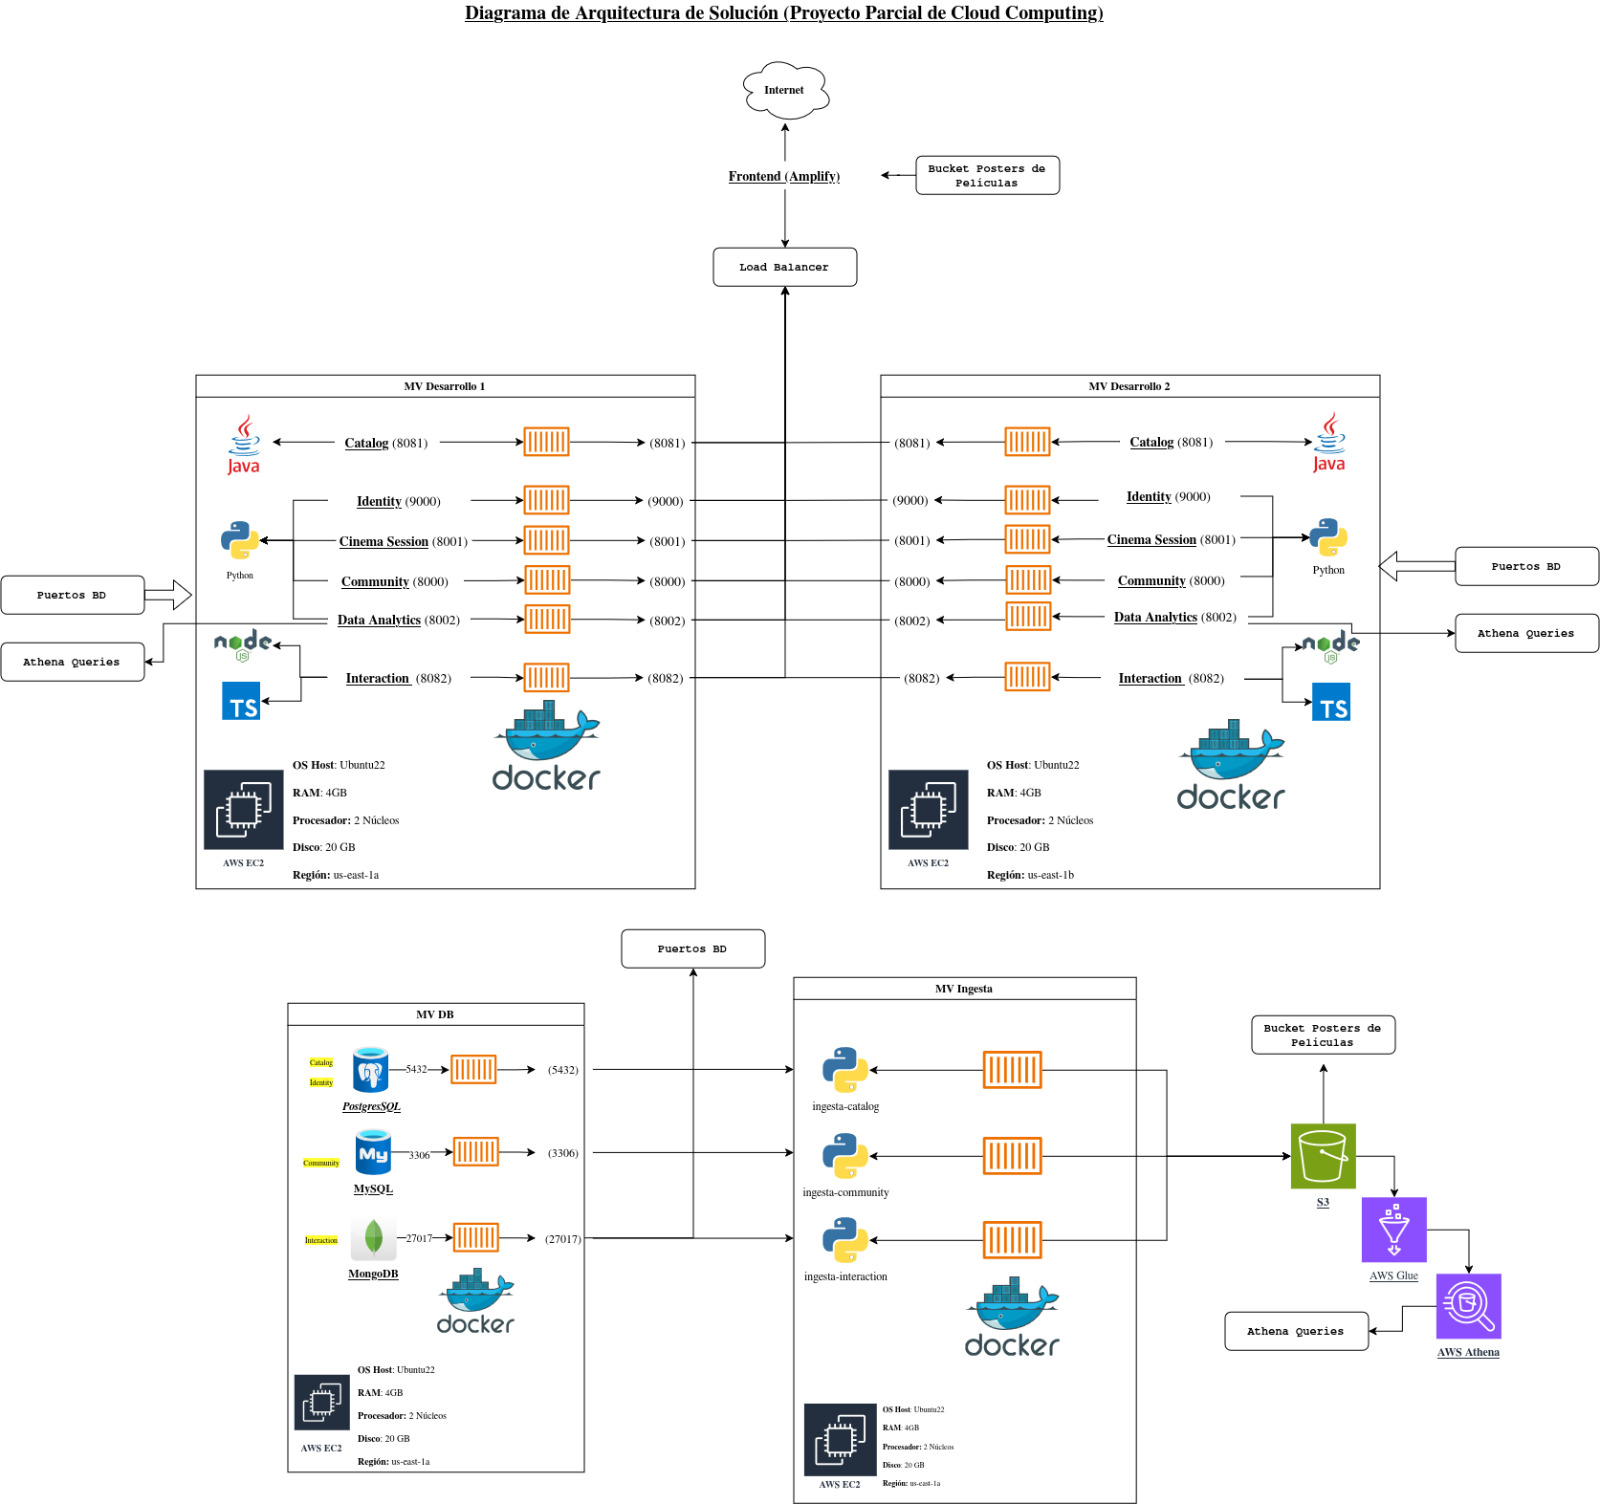
\includegraphics[width=\textwidth]{figures/arquitectura-general.jpeg}\caption{Arquitectura general de ASTRA CLOUD}\label{fig:arquitectura_general}\end{figure}
\section{Ruta de acceso}
Las solicitudes del cliente llegan primero a API Gateway y pasan al ALB interno mediante VPC Link. El balanceador las dirige a la instancia EC2 y al contenedor donde se ejecuta el servicio correspondiente. El ALB reparte las solicitudes entre las instancias disponibles y no queda expuesto directamente a Internet.
